\documentclass[11pt,a4paper]{article}

% ---------------------------------------------------------------- packages
\usepackage[margin=1in]{geometry}
\usepackage[T1]{fontenc}
\usepackage{lmodern}
\usepackage{microtype}
\usepackage{amsmath,amssymb,amsthm}
\usepackage{booktabs}
\usepackage{tabularx}
\usepackage{array}
\usepackage{graphicx}
\usepackage[table]{xcolor}
\usepackage{tikz}
\usetikzlibrary{arrows.meta,positioning}
\usepackage{pgfplots}
\pgfplotsset{compat=1.18}
\usepackage{algorithm}
\usepackage{algpseudocode}
\usepackage{enumitem}
\usepackage[section]{placeins}
\usepackage[font=small,labelfont=bf]{caption}
\usepackage[numbers,sort&compress]{natbib}
\usepackage[hidelinks]{hyperref}

\definecolor{smlindigo}{HTML}{4F46E5}
\definecolor{smlcyan}{HTML}{06B6D4}
\definecolor{smlslate}{HTML}{94A3B8}
\definecolor{smlamber}{HTML}{F59E0B}
\definecolor{smlred}{HTML}{DC2626}
\definecolor{smlgreen}{HTML}{059669}

\newtheorem{definition}{Definition}
\newtheorem{proposition}{Proposition}
\newtheorem{corollary}{Corollary}
\theoremstyle{remark}
\newtheorem*{remark}{Remark}

\newcommand{\sys}{SML}
\newcommand{\best}[1]{\textbf{#1}}
\newcommand{\vis}{\mathcal{V}}
\newcommand{\topk}{\mathrm{top}_k}
\newcolumntype{Y}{>{\raggedright\arraybackslash}X}
\setlist{itemsep=2pt,topsep=4pt}
\makeatletter
\setlength{\@fptop}{0pt}\setlength{\@fpsep}{2.5em}\setlength{\@fpbot}{0pt plus 1fil}
\makeatother

\title{\textbf{Similarity Is Not Authorisation:\\
Need-to-Know Collective Memory for Multi-Team LLM Agents}}

\author{
  {[Student Name]}\thanks{Replace the bracketed placeholders with the author details before submission.}\\
  \small Department of Computer Science and Engineering, {[Institute Name]}\\
  \small \texttt{{[student-email]}}
  \and
  {[Guide Name]}\\
  \small Department of Computer Science and Engineering, {[Institute Name]}\\
  \small \texttt{{[guide-email]}}
}
\date{}

\begin{document}
\maketitle

% ================================================================ abstract
\begin{abstract}
Organisations now run fleets of LLM agents, one per team, each with a private memory. Pooling those
memories promises that no team re-derives what another already knows---but a shared memory is searched by
\emph{similarity}, and similarity is not authorisation. We formalise the requirement as \emph{retrieval
non-interference} (RNI): everything a principal observes from a memory search---which items, in what order,
with what scores, and how many---must be a function of the memories it may read. We prove that the
prevailing \emph{rank-then-filter} design violates RNI through the \emph{number} of results it returns, and
that hybrid retrieval with index-wide lexical statistics violates it through \emph{scores} even when every
returned item is authorised; \emph{authorise-before-rank} with document-local scoring satisfies it. We build
\sys{}, a governed collective memory for agents on this principle: one access predicate compiled into
application, SQL and vector-index form, document-local hybrid scoring, a defence-in-depth re-check,
immutable versions, contradiction review and an append-only audit trail, reachable over REST, SDKs and the
Model Context Protocol. Controlled experiments confirm the analysis: when ten teams hold topically overlapping
knowledge and half of it is private, rank-then-filter answers @@E1:scifact:0.5:post1_short:pct@@ of queries with a
truncated list---each revealing that similar hidden memories exist---and it still does so for
@@E1:locomo:1.0:post1_short:pct@@ of queries when teams' knowledge is topically disjoint; index-wide BM25 changed the
scores of visible results in @@E2:bm25_global_score_of_visible_results_changed:pct@@ and their order in
@@E2:bm25_global_top10_order_changed:pct@@ of cases when only hidden memories changed; and filtered HNSW matched exact
authorise-before-rank on every query at no measurable cost. End to end, 0 of 140
adversarial attempts leaked, sharing raised cross-team Hit@1 from 0.35 to 0.975, and on LoCoMo, LongMemEval and
BEIR \sys{} outperformed BM25 and a plain vector store (Recall@10 0.673 and 0.807; nDCG@10 0.718 and 0.359),
matching the benchmark authors' DRAGON retriever with a 33M-parameter local model at 83--109\,ms median latency.
Answers that an open 8B model wrote from \sys{}'s memories were judged correct for
@@QA:sml_hybrid:accuracy:pct@@ of @@QA:n@@ sampled LoCoMo questions, against @@QA:bm25:accuracy:pct@@ with BM25,
@@QA:dense:accuracy:pct@@ with a plain vector store (@@QA:p:dense@@) and @@QA:none:accuracy:pct@@ without memory.
\end{abstract}

% ================================================================ 1 introduction
\section{Introduction}

AI agents now write code, test releases, triage security findings and answer customers. They are
typically configured per team, and each keeps its own memory: a conversation log, a scratch file, a private
vector index. When the Development agent learns that sign-ins fail because refresh tokens expire, the QA agent
that meets the same symptom a week later cannot benefit from it; it re-investigates, pays for the same
reasoning again, and may record a different conclusion. In our in-house study, agents restricted to their
own memory had to re-derive 62.5\,\% of the answers the organisation already held (Section~\ref{sec:rq4}).

The obvious remedy is a single shared memory. It is also where the difficulty begins. Memory retrieval
ranks \emph{everything in the index} by similarity to the query, and a Support agent asking why PDF export
fetches internal URLs is, by construction, closest to the Security team's confidential server-side request
forgery finding. \emph{Similarity is not authorisation.} The common engineering answer---retrieve the top
candidates, then drop the ones the caller may not read---looks safe, because no forbidden item is ever
returned. We show that it is not: the \emph{number} of results it returns depends on memories the caller
cannot see, which turns every search into an oracle for the existence of hidden knowledge, and it silently
loses the caller's own relevant memories when hidden ones crowd the candidate list. Hybrid retrieval adds a
second, subtler channel: lexical scores such as BM25 use collection-wide statistics, so the \emph{scores and
order} of perfectly authorised results move when hidden memories change---the same class of leak B{\"u}ttcher and
Clarke demonstrated for multi-user file-system search two decades ago~\cite{buettcher2005security}.

This paper makes the requirement precise and builds a system that meets it.
\begin{enumerate}[leftmargin=*]
  \item \textbf{A security property for memory retrieval.} We define \emph{retrieval non-interference} (RNI),
  an adaptation of non-interference~\cite{goguen1982noninterference} to ranked retrieval, and prove that
  authorise-before-rank with document-local scoring satisfies it, rank-then-filter violates it through result
  counts, and index-wide scoring statistics violate it through scores (Section~\ref{sec:rni}).
  \item \textbf{\sys{}, a governed collective memory for agents.} One access predicate over five visibility
  levels is compiled into application code, a SQL predicate and a vector-index filter; hybrid dense and
  full-text retrieval uses only document-local scores; every candidate is re-checked against the system of
  record; knowledge is versioned, contradictions are routed to human review, and every access and refusal is
  written to an append-only log. Agents connect over REST, SDKs and the Model Context
  Protocol~\cite{anthropic2024mcp} (Section~\ref{sec:design}).
  \item \textbf{Controlled experiments on the placement of authorisation}: recall starvation and short-list
  rates of rank-then-filter on two multi-tenant corpora, the statistics side channel of index-wide BM25, and
  the fidelity and cost of filtered approximate search (Sections~\ref{sec:rq1}--\ref{sec:rq2}).
  \item \textbf{An end-to-end evaluation}: an adversarial suite of 140 attacks, end-to-end answer accuracy with an
  LLM judge, an in-house cross-team
  benchmark, and three public benchmarks (LoCoMo~\cite{maharana2024locomo}, LongMemEval~\cite{wu2025longmemeval},
  BEIR~\cite{thakur2021beir}) against BM25, a plain vector store and published results of other memory layers
  (Sections~\ref{sec:rq3}--\ref{sec:rq7}).
\end{enumerate}
The implementation, the benchmark harnesses and all raw results are released with the project.

% ================================================================ 2 background
\section{Background and Threat Model}
\label{sec:background}

\paragraph{Agent memory today.} Research systems give a single agent long-term memory by retrieval over an
event stream~\cite{park2023generative} or by paging context in and out of the prompt~\cite{packer2023memgpt}.
Production memory layers---Mem0~\cite{chhikara2025mem0}, Zep~\cite{rasmussen2025zep},
LangMem~\cite{langmem2025}, A-Mem~\cite{xu2025amem}---extract facts or temporal knowledge graphs with an LLM
and are evaluated by the answer accuracy they enable on long conversations. Their unit of isolation is a
user, agent or project identifier: memory is either wholly private to that scope or wholly visible within it.
Organisation-wide sharing with per-memory need-to-know rules, and the leakage it can cause, is outside their
design and their evaluations.

\paragraph{Principals, memories and policy.} An organisation has teams. A \emph{principal} $p$ is an agent
(authenticated by its own API key) or a human user; it belongs to at most one team $\tau(p)$ and holds roles
that grant permissions such as \texttt{memory:create}, \texttt{memory:read} or \texttt{memory:share}. A
\emph{memory} $m$ has content, a type, tags, importance and confidence in $[0,1]$, an owning team $\tau(m)$,
a creator $c(m)$, a visibility $v(m)$, a sensitivity level, an optional expiry, explicit grants to teams
$G_T(m)$ and agents $G_A(m)$, and a version history. Visibility is one of \texttt{private}, \texttt{team},
\texttt{selected\_teams}, \texttt{selected\_agents} or \texttt{organization} (Appendix, Table~\ref{tab:visibility});
confidential and restricted memories may not be organisation-wide. For a non-administrator holding
\texttt{memory:read}, an active, unexpired memory is readable, $R(p,m)$, if and only if
\begin{equation}
\begin{split}
& c(m) = p \;\lor\; v(m) = \texttt{organization} \\
& \lor\; \Big( v(m) \neq \texttt{private} \;\land\; \big[ \big(\tau(p) = \tau(m) \land v(m) \in \{\texttt{team}, \texttt{selected\_teams}\}\big) \\
& \qquad\qquad \lor\; \tau(p) \in G_T(m) \;\lor\; p \in G_A(m) \big] \Big).
\end{split}
\label{eq:read}
\end{equation}
Modifying a memory additionally requires its creator or a manager of the owning team.

\paragraph{Threat model.} The adversary is an authenticated but unauthorised principal: an agent of
another team, or a compromised agent, that issues arbitrary API requests. It may search with any text,
including the exact title or content of a memory it wants (the strongest similarity attack), probe the system
repeatedly, attempt to update, version-browse or share memories to itself, and attempt privilege escalation
(creating teams or agents, reading the audit log, listing users, re-indexing). It observes everything the
API returns: result lists, their lengths, scores, errors and warnings. Timing side channels, compromise of the
database or host, and poisoning of shared knowledge by authorised writers~\cite{zou2025poisonedrag} are out
of scope; the latter is mitigated but not prevented by provenance, verification and contradiction review.

% ================================================================ 3 RNI
\section{Retrieval Non-Interference}
\label{sec:rni}

\subsection{Definitions}

Let $S$ be the set of stored memories and $\vis_p(S) = \{ m \in S : R(p,m) \}$ the memories principal $p$ may
read. A retrieval mechanism $F$ maps a principal, a query $q$ and the store to an observable response
$F(p,q,S)$: an ordered list of memories with scores (and hence a length). A scoring function $s(q,m)$ is
\emph{document-local} if its value depends only on $q$ and on attributes of $m$ itself, and not on any other
memory in $S$. Cosine similarity of embeddings, PostgreSQL's \texttt{ts\_rank\_cd}, importance, confidence and
verification status are document-local; BM25~\cite{robertson2009bm25} is not, because its inverse document
frequency and length normalisation are computed over a collection.

\begin{definition}[Confidentiality of content]
$F$ is \emph{content-confidential} if $F(p,q,S) \subseteq \vis_p(S)$ for every $p$, $q$ and $S$.
\end{definition}

\begin{definition}[Retrieval non-interference]
$F$ satisfies \emph{retrieval non-interference} (RNI) if for every principal $p$, query $q$ and pair of stores
$S, S'$ with $\vis_p(S) = \vis_p(S')$, the responses are identical: $F(p,q,S) = F(p,q,S')$, including order,
scores and length.
\end{definition}

RNI is the retrieval analogue of Goguen--Meseguer non-interference~\cite{goguen1982noninterference,sabelfeld2003language}:
changing what $p$ cannot see must not change what $p$ observes. Content confidentiality is necessary but, as
we show, far from sufficient.

Figure~\ref{fig:placements} shows three placements of authorisation relative to ranking, with $\topk$
selecting the $k$ highest-scoring memories (ties broken by a fixed memory order):
\begin{align*}
F_{\mathrm{none}}(p,q,S) &= \topk(s, S), \\
F_{\mathrm{post}}^{\,n}(p,q,S) &= \topk\big(s,\; \mathrm{top}_n(s,S) \cap \vis_p(S)\big) \qquad (n \geq k), \\
F_{\mathrm{pre}}(p,q,S) &= \topk\big(s,\; \vis_p(S)\big).
\end{align*}

\begin{figure}[htbp]
\centering
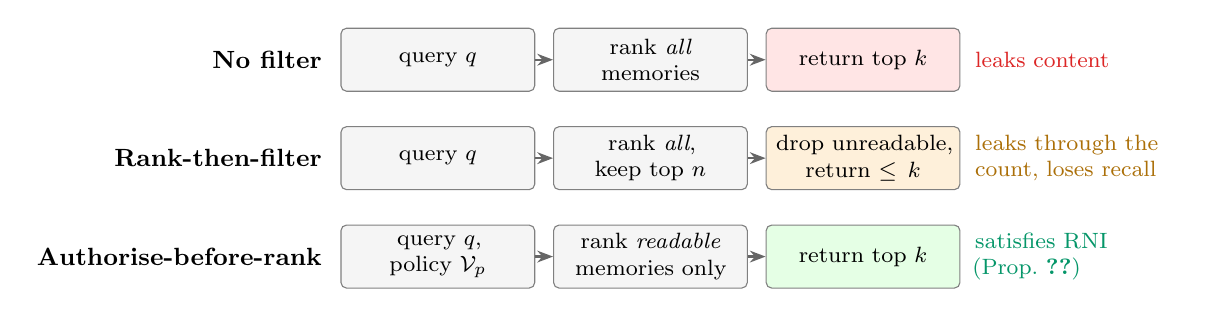
\begin{tikzpicture}[
  st/.style={draw=black!50, rounded corners=2pt, align=center, font=\footnotesize, minimum height=0.8cm, inner sep=3pt, text width=2.25cm, fill=#1, execute at begin node={\hyphenpenalty=10000\exhyphenpenalty=10000}},
  st/.default=white,
  arr/.style={-{Stealth[length=2mm]}, thick, black!60},
  lab/.style={font=\small\bfseries, anchor=east, align=right},
  outc/.style={font=\footnotesize, anchor=west, align=left, text width=2.7cm}]
\node[lab] at (-0.3,0) {No filter};
\node[st=gray!8] (a1) at (1.05,0) {query $q$};
\node[st=gray!8] (a2) at (3.75,0) {rank \emph{all} memories};
\node[st=red!10] (a3) at (6.45,0) {return top $k$};
\node[outc, text=smlred] at (7.75,0) {leaks content};
\draw[arr] (a1) -- (a2); \draw[arr] (a2) -- (a3);
\node[lab] at (-0.3,-1.25) {Rank-then-filter};
\node[st=gray!8] (b1) at (1.05,-1.25) {query $q$};
\node[st=gray!8] (b2) at (3.75,-1.25) {rank \emph{all}, keep top $n$};
\node[st=smlamber!15] (b3) at (6.45,-1.25) {drop unreadable, return $\le k$};
\node[outc, text=smlamber!70!black] at (7.75,-1.25) {leaks through the count, loses recall};
\draw[arr] (b1) -- (b2); \draw[arr] (b2) -- (b3);
\node[lab] at (-0.3,-2.5) {Authorise-before-rank};
\node[st=gray!8] (c1) at (1.05,-2.5) {query $q$, policy $\vis_p$};
\node[st=gray!8] (c2) at (3.75,-2.5) {rank \emph{readable} memories only};
\node[st=green!10] (c3) at (6.45,-2.5) {return top $k$};
\node[outc, text=smlgreen] at (7.75,-2.5) {satisfies RNI (Prop.~\ref{prop:pre})};
\draw[arr] (c1) -- (c2); \draw[arr] (c2) -- (c3);
\end{tikzpicture}
\caption{Three placements of authorisation in memory retrieval.}
\label{fig:placements}
\end{figure}

\subsection{Results}

\begin{proposition}[Authorise-before-rank]
\label{prop:pre}
If $s$ is document-local, $F_{\mathrm{pre}}$ is content-confidential and satisfies RNI.
\end{proposition}
\begin{proof}
$F_{\mathrm{pre}}$ selects from $\vis_p(S)$ only, so it is content-confidential. Its output is determined by
the set $\vis_p(S)$, the scores $s(q,m)$ for $m \in \vis_p(S)$ and the fixed tie-breaking order. Because $s$ is
document-local, each score depends on $q$ and $m$ alone. Hence if $\vis_p(S)=\vis_p(S')$ the candidate sets and
all their scores coincide, and so do the selected lists, their order, scores and length.
\end{proof}

\begin{proposition}[Rank-then-filter]
\label{prop:post}
$F_{\mathrm{post}}^{\,n}$ is content-confidential but, for every finite depth $n \geq k$, violates RNI: there exist
stores $S, S'$ with $\vis_p(S)=\vis_p(S')$ whose responses differ in length.
\end{proposition}
\begin{proof}
Content confidentiality holds because the output is a subset of $\vis_p(S)$. Let $S$ contain at least $k$
memories, all readable by $p$, so that $F_{\mathrm{post}}^{\,n}(p,q,S)$ has length $k$. Let $S' = S \cup H$, where $H$
consists of $n-k+1$ memories hidden from $p$ that score higher on $q$ than every memory of $S$ (for instance
paraphrases of $q$ written by another team). Then $\vis_p(S')=\vis_p(S)$, but $\mathrm{top}_n(s,S')$ consists of $H$ and
only $k-1$ readable memories, so $F_{\mathrm{post}}^{\,n}(p,q,S')$ has length $k-1$.
\end{proof}

\begin{corollary}[Existence oracle and recall starvation]
Under rank-then-filter, an unauthorised principal learns whether hidden memories similar to a query of its
choice exist by observing a short result list; and readable memories that would rank in the top $k$ among
$\vis_p(S)$ are dropped whenever hidden memories occupy the first $n$ ranks. Over-fetching (larger $n$) raises the
number of similar hidden memories needed to trigger either effect, but no finite $n$ removes them.
\end{corollary}

\begin{proposition}[Collection statistics]
\label{prop:stats}
If $s$ depends on statistics of $S$ that include hidden memories---inverse document frequency, average length,
or normalisation by the maximum score over $S$---then even $F_{\mathrm{pre}}$ can violate RNI: responses are
content-confidential but their scores and order depend on hidden memories.
\end{proposition}
\begin{proof}
For BM25, the weight of term $t$ is $\log\!\big(1 + (N - \mathrm{df}_t + 0.5)/(\mathrm{df}_t + 0.5)\big)$ with $N$ and
$\mathrm{df}_t$ counted over $S$. Adding hidden memories containing $t$ changes $\mathrm{df}_t$ and $N$, hence the
score of every readable memory containing $t$, although $\vis_p(S)$ is unchanged; with several query terms the
relative weights shift and the order of readable memories can change.
\end{proof}

B{\"u}ttcher and Clarke showed that such statistics are exploitable: in multi-user file search, relevance
scores computed over a system-wide index let a user infer the content of files it cannot
read~\cite{buettcher2005security}. Proposition~\ref{prop:stats} says the same channel re-appears in hybrid
agent memory whenever the lexical component is BM25 over the shared index---the default in many hybrid
search engines.

\begin{remark}[Approximate search]
Graph indexes such as HNSW~\cite{malkov2020hnsw} traverse hidden vectors while answering a filtered query;
filtered traversal~\cite{gollapudi2023filtered,patel2024acorn} returns only matching vectors, so content
confidentiality holds, but the approximation error can in principle depend on the hidden part of the graph.
Proposition~\ref{prop:pre} is exact for exhaustive search; we measure how closely filtered HNSW matches it
in Section~\ref{sec:rq1}.
\end{remark}

\begin{remark}[Declassification]
A system may deliberately release a bounded amount of information about hidden memories. \sys{} does so at
exactly one point: when a new memory contradicts one its author cannot read, the author learns only the
\emph{count} of such conflicts, the details go to administrators, and the event is audited.
\end{remark}

% ================================================================ 4 design
\section{\sys{}: Design}
\label{sec:design}

\sys{} is built so that every path to a memory realises $F_{\mathrm{pre}}$ with document-local scores.

\subsection{Architecture}

Figure~\ref{fig:arch} shows the components. Every request passes one gateway that authenticates it (a
JWT~\cite{rfc7519} or an agent API key) and authorises it twice: role-based access control~\cite{sandhu1996rbac}
decides whether the operation is permitted, and the read predicate~\eqref{eq:read}---an attribute-based
rule~\cite{hu2014abac}---decides whether the specific memory may be touched. PostgreSQL is the system of
record for memories, versions, grants, identities and the audit log; Qdrant~\cite{qdrant2024} stores one vector
per memory with the payload fields the predicate needs; embeddings are computed locally with
\texttt{bge-small-en-v1.5}~\cite{xiao2023cpack} (384 dimensions, 33M parameters), so no text leaves the deployment.

\begin{figure}[htbp]
\centering
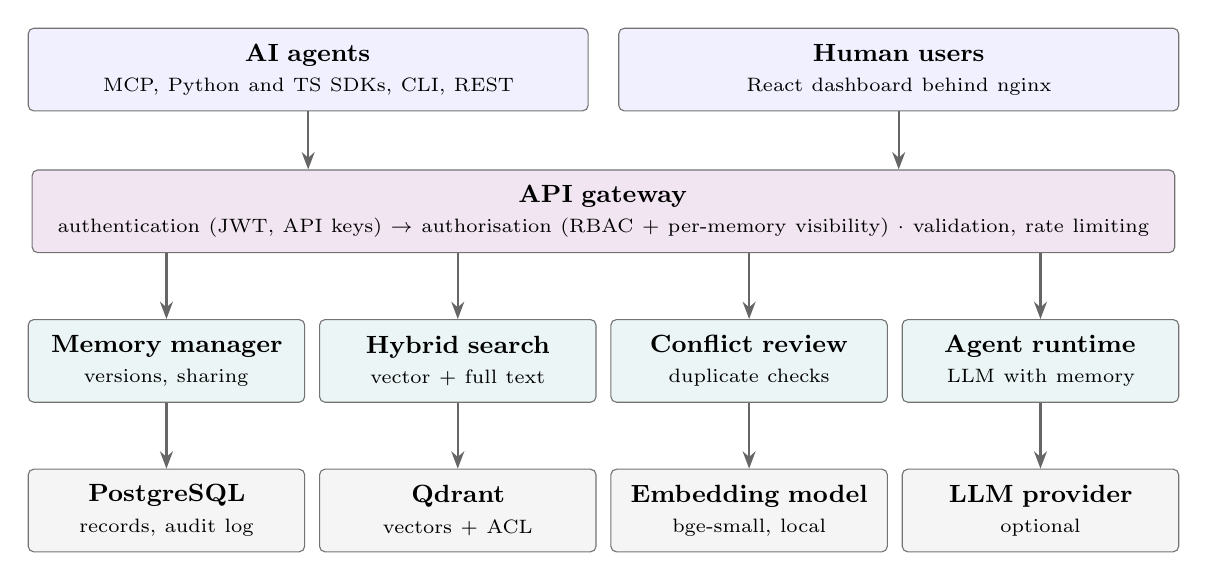
\begin{tikzpicture}[
  box/.style={draw=black!55, rounded corners=2pt, align=center, font=\small, inner sep=3pt, minimum height=1.05cm, fill=#1, execute at begin node={\hyphenpenalty=10000\exhyphenpenalty=10000}},
  box/.default=white,
  arr/.style={-{Stealth[length=2.2mm]}, thick, black!60}]
\node[box=blue!6, text width=6.9cm] (agents) at (-3.75,0) {\textbf{AI agents}\\\scriptsize MCP, Python and TS SDKs, CLI, REST};
\node[box=blue!6, text width=6.9cm] (humans) at (3.75,0) {\textbf{Human users}\\\scriptsize React dashboard behind nginx};
\node[box=violet!10, text width=14.3cm] (gw) at (0,-1.8) {\textbf{API gateway}\\\scriptsize authentication (JWT, API keys) $\rightarrow$ authorisation (RBAC + per-memory visibility) $\cdot$ validation, rate limiting};
\node[box=teal!8, text width=3.3cm] (s1) at (-5.55,-3.7) {\textbf{Memory manager}\\\scriptsize versions, sharing};
\node[box=teal!8, text width=3.3cm] (s2) at (-1.85,-3.7) {\textbf{Hybrid search}\\\scriptsize vector + full text};
\node[box=teal!8, text width=3.3cm] (s3) at (1.85,-3.7) {\textbf{Conflict review}\\\scriptsize duplicate checks};
\node[box=teal!8, text width=3.3cm] (s4) at (5.55,-3.7) {\textbf{Agent runtime}\\\scriptsize LLM with memory};
\node[box=gray!8, text width=3.3cm] (d1) at (-5.55,-5.6) {\textbf{PostgreSQL}\\\scriptsize records, audit log};
\node[box=gray!8, text width=3.3cm] (d2) at (-1.85,-5.6) {\textbf{Qdrant}\\\scriptsize vectors + ACL};
\node[box=gray!8, text width=3.3cm] (d3) at (1.85,-5.6) {\textbf{Embedding model}\\\scriptsize bge-small, local};
\node[box=gray!8, text width=3.3cm] (d4) at (5.55,-5.6) {\textbf{LLM provider}\\\scriptsize optional};
\draw[arr] (agents.south) -- (agents.south |- gw.north);
\draw[arr] (humans.south) -- (humans.south |- gw.north);
\foreach \x in {s1,s2,s3,s4} { \draw[arr] (\x.north |- gw.south) -- (\x.north); }
\draw[arr] (s1.south) -- (d1.north);
\draw[arr] (s2.south) -- (d2.north);
\draw[arr] (s3.south) -- (d3.north);
\draw[arr] (s4.south) -- (d4.north);
\end{tikzpicture}
\caption{Architecture of \sys{}. Every path to a memory passes authentication and two-level authorisation;
audit records are written in an independent transaction.}
\label{fig:arch}
\end{figure}

\subsection{One predicate, three enforcement points}
\label{sec:access}

The read predicate~\eqref{eq:read} exists in three synchronised forms, and tests assert that they agree:
\texttt{can\_read} evaluates a concrete PostgreSQL row and is authoritative; \texttt{sql\_read\_filter} is the
same rule as a SQL predicate for listings and full-text search; \texttt{build\_read\_filter} expresses it as a
Qdrant payload filter---a disjunction of conjunctions over visibility, owning team, creator, grants, status and
expiry---that is pushed \emph{into} the nearest-neighbour query. Similarity search therefore ranks only readable
memories ($F_{\mathrm{pre}}$). Every candidate is then re-checked with \texttt{can\_read} against the current row,
which protects against a stale vector payload after a permission change and against a bug in either filter.

\subsection{Document-local hybrid retrieval}
\label{sec:retrieval}

Embeddings capture paraphrase but blur exact identifiers such as error codes, CVE numbers and ticket ids. \sys{}
adds a PostgreSQL full-text path~\cite{postgres2023fts} (Algorithm~\ref{alg:search}): a generated, weighted \texttt{tsvector} over title and content,
queried with \texttt{websearch\_to\_tsquery} under the SQL form of the same predicate, in which every query term
must match. Both paths use only document-local signals, as Proposition~\ref{prop:stats} requires:
\begin{equation}
s(m) = 0.90\,\mathrm{sim}(q,m) + 0.05\,\mathrm{imp}(m) + 0.05\,\mathrm{conf}(m) + 0.02\,[\mathrm{verified}(m)] + 0.10\,\mathrm{kw}(q,m),
\label{eq:score}
\end{equation}
where $\mathrm{sim}$ is cosine similarity (computed from Qdrant for keyword-only candidates too) and $\mathrm{kw}$ is
\texttt{ts\_rank\_cd}---a cover-density rank that uses no collection statistics---normalised by the best keyword
score among the \emph{readable} candidates. The weights favour meaning, let verified and high-confidence knowledge win
ties, and reward exact matches. If the vector store is unreachable, search degrades to permission-filtered keyword
search instead of failing.

\begin{algorithm}[htbp]
\caption{Permission-aware hybrid search ($F_{\mathrm{pre}}$ with document-local scores)}
\label{alg:search}
\begin{algorithmic}[1]
\Require principal $p$, query $q$, metadata filters $F$, result size $k$
\State $\phi \gets \textsc{ReadFilter}(p) \land F$ \Comment{visibility, grants, status, expiry, type, project, \dots}
\State $C_{\mathrm{kw}} \gets$ full-text matches of $q$ in PostgreSQL under $\phi$ (all terms), ranked by \texttt{ts\_rank\_cd}
\State $\mathbf{v} \gets \textsc{Embed}(q)$
\State $C_{\mathrm{vec}} \gets$ the $3k$ nearest neighbours of $\mathbf{v}$ in Qdrant under $\phi$
\State $C \gets C_{\mathrm{kw}} \cup C_{\mathrm{vec}}$; obtain cosine similarity for keyword-only candidates
\ForAll{$m \in C$}
  \If{\textbf{not} \textsc{CanRead}$(p, m)$ on the current PostgreSQL row}
    \State remove $m$ from $C$ \Comment{defence in depth}
  \EndIf
  \State compute $s(m)$ with Equation~\eqref{eq:score}
\EndFor
\State update access and cross-team reuse counters; append a \texttt{MEMORY\_SEARCH} audit record
\State \Return the $k$ highest-scoring memories of $C$
\end{algorithmic}
\end{algorithm}

\subsection{Governance of shared knowledge}
\label{sec:lifecycle}

\paragraph{Writes.} A new memory is validated, authorised (\texttt{memory:create}; the body may not name another
agent or team), embedded and checked against \emph{readable} memories for duplicates (identical content hash, or
cosine similarity $\geq 0.92$). Organisation-wide candidates with similarity $\geq 0.70$ are passed to contradiction
rules (e.g.\ different numeric values or opposing technology choices for the same subject), which open a conflict
for human review; this is the declassification point of Section~\ref{sec:rni}. The row, version~1 and grants are
flushed to PostgreSQL, the vector is upserted, and the transaction commits; if the commit fails the vector is
deleted, and an administrator endpoint detects and repairs any divergence by re-embedding from PostgreSQL.

\paragraph{Versions and provenance.} Updates lock the row, check an optional expected version, and store an
immutable snapshot linked to its predecessor; there is one vector per memory, so search always returns the latest
version. Humans resolve conflicts with \emph{keep new}, \emph{keep existing}, \emph{keep both} or \emph{dismiss};
nothing is overwritten silently.

\paragraph{Accountability.} Logins, token events, every memory operation, sharing and role changes, conflict
resolutions and every denial are recorded with actor, team, on-behalf-of principal, resource, outcome, reason and
request identifier. Audit records are written in an independent transaction, so refused operations are always
recorded, and a database trigger rejects \texttt{UPDATE} and \texttt{DELETE} on the audit table.

\paragraph{Identity.} Passwords are hashed with Argon2id~\cite{biryukov2016argon2}; access tokens live 15 minutes;
refresh tokens rotate on every use and re-use revokes the whole token family; agent API keys are stored only as
keyed hashes; authentication is rate limited with temporary lock-out.

\subsection{Agent interfaces}

\begin{sloppypar}
Agents reach \sys{} through a REST API (57 operations), a Model Context Protocol endpoint exposing eight tools
(\texttt{search\_memory}, \texttt{remember}, \texttt{get\_memory}, \texttt{update\_memory}, \texttt{share\_memory},
\texttt{memory\_history}, \texttt{list\_teams}, \texttt{whoami}) that off-the-shelf MCP clients can use without code,
and Python and TypeScript SDKs with a command-line tool, bulk import and LLM tool definitions. All interfaces act as
the calling agent through the same services, so authorisation and auditing are identical on every path.
\end{sloppypar}

% ================================================================ 5 implementation
\section{Implementation}
\label{sec:impl}

\sys{} is written in Python~3.12 with FastAPI (API), SQLAlchemy~2 and Alembic (PostgreSQL~16 schema with foreign keys,
check constraints, a generated full-text column and the append-only audit trigger), Qdrant~1.13 with payload indexes on
every filtered field, and fastembed/ONNX for local embeddings. A React dashboard provides monitoring, a memory explorer,
access management, the audit log, conflict review and an \emph{agent playground} in which a human acts as an agent
under that agent's permissions, audited on the human's behalf. The system runs as four containers from one
\texttt{docker compose} command. Its test suite---105 backend tests against real PostgreSQL, Qdrant and the embedding
model (including an end-to-end MCP test with the official client), 14 Python and 5 TypeScript SDK tests, and a 16-step
acceptance scenario against the running deployment---passes.

% ================================================================ 6 evaluation
\section{Evaluation}
\label{sec:eval}

We ask seven questions. \textbf{RQ1:} where should authorisation happen---what do rank-then-filter and filtered
approximate search cost? \textbf{RQ2:} do index-wide ranking statistics leak? \textbf{RQ3:} is \sys{} secure end to end?
\textbf{RQ4:} does shared memory help agents? \textbf{RQ5:} how good is \sys{}'s retrieval on public benchmarks, and how
does it compare with other memory layers? \textbf{RQ6:} does better retrieval yield more correct answers?
\textbf{RQ7:} what does governed retrieval cost?

\paragraph{Setup.} All experiments ran on one laptop (Windows~11 on ARM64, Docker Desktop with 12 virtual CPUs and
15.5\,GB of memory, no GPU). RQ1--RQ2 are controlled experiments with the system's embedding model and exact cosine
search (and Qdrant for filtered HNSW). RQ3--RQ7 exercise the running system through its public API; the public
benchmarks ran against a second API process with its own database and collection, so 100{,}000+ benchmark memories did
not touch the demonstration data. Two baselines ran over exactly the same texts: \textbf{BM25} ($k_1{=}1.5$, $b{=}0.75$)
and a \textbf{plain vector store} using \texttt{all-MiniLM-L6-v2}~\cite{wang2020minilm,reimers2019sbert}, the default
embedding model of Chroma-style memories. Published results of other systems are quoted, not re-run.

\paragraph{Validity checks.} Our local \texttt{all-MiniLM-L6-v2} baseline reproduces its published BEIR scores exactly
(nDCG@10 0.645 on SciFact and 0.316 on NFCorpus~\cite{muennighoff2023mteb}); \sys{}'s dense mode reproduces the published
scores of \texttt{bge-small-en-v1.5} (0.717 vs.\ 0.713; 0.342 vs.\ 0.343); our LongMemEval metrics, ported line by line
from the official code, agree with it to $10^{-16}$ on 3{,}000 randomised rankings; and retrieval is deterministic---two
independent LoCoMo runs produced identical recall.

\subsection{RQ1: Where should authorisation happen?}
\label{sec:rq1}

\paragraph{Design.} We turn two corpora into multi-tenant memories with ten teams. In \emph{LoCoMo-MT}, each of the
10 LoCoMo conversations (5{,}882 turns, 1{,}535 questions) belongs to its own team and every question is asked by the team
that owns its conversation: teams hold \emph{topically disjoint} knowledge. In \emph{SciFact-MT}, the 5{,}183 abstracts
and 300 claims of BEIR SciFact are assigned to teams uniformly at random: teams hold \emph{topically overlapping}
knowledge, as departments of one organisation do. A fraction $\rho$ of every other team's memories is private to that
team; the rest is organisation-visible. We compare $F_{\mathrm{pre}}$, $F_{\mathrm{post}}^{\,n}$ with over-fetch
$n=\alpha k$ for $\alpha\in\{1,2,5,10\}$, and $F_{\mathrm{none}}$, all with $k=10$ and exact cosine search, over three
random seeds. Recall@10 is measured against the evidence the asker may read.

\begin{figure}[htbp]
\centering
\begin{minipage}{0.49\textwidth}
\centering
\begin{tikzpicture}
\begin{axis}[
  width=0.8\linewidth, height=5.6cm,
  xlabel={$\rho$ (private share of other teams' memories)},
  ylabel={Recall@10 (readable evidence)},
  xtick={0,0.25,0.5,0.75,1}, xticklabel style={/pgf/number format/fixed},
  ymin=0.8, ymax=1.02, grid=major, grid style={gray!25},
  legend style={font=\scriptsize, at={(0.5,-0.3)}, anchor=north, legend columns=2, draw=none}, legend cell align=left,
  label style={font=\small}, tick label style={font=\scriptsize},
]
\addplot[smlindigo, very thick, mark=*] coordinates {(0,@@E1:scifact:0.0:pre_recall@@) (0.25,@@E1:scifact:0.25:pre_recall@@) (0.5,@@E1:scifact:0.5:pre_recall@@) (0.75,@@E1:scifact:0.75:pre_recall@@) (1,@@E1:scifact:1.0:pre_recall@@)};
\addplot[smlcyan, thick, mark=square*] coordinates {(0,@@E1:scifact:0.0:post10_recall@@) (0.25,@@E1:scifact:0.25:post10_recall@@) (0.5,@@E1:scifact:0.5:post10_recall@@) (0.75,@@E1:scifact:0.75:post10_recall@@) (1,@@E1:scifact:1.0:post10_recall@@)};
\addplot[smlamber, thick, mark=triangle*] coordinates {(0,@@E1:scifact:0.0:post2_recall@@) (0.25,@@E1:scifact:0.25:post2_recall@@) (0.5,@@E1:scifact:0.5:post2_recall@@) (0.75,@@E1:scifact:0.75:post2_recall@@) (1,@@E1:scifact:1.0:post2_recall@@)};
\addplot[smlred, thick, mark=diamond*] coordinates {(0,@@E1:scifact:0.0:post1_recall@@) (0.25,@@E1:scifact:0.25:post1_recall@@) (0.5,@@E1:scifact:0.5:post1_recall@@) (0.75,@@E1:scifact:0.75:post1_recall@@) (1,@@E1:scifact:1.0:post1_recall@@)};
\legend{authorise-before-rank, rank-then-filter $n{=}10k$, rank-then-filter $n{=}2k$, rank-then-filter $n{=}k$}
\end{axis}
\end{tikzpicture}
\end{minipage}\hfill
\begin{minipage}{0.49\textwidth}
\centering
\begin{tikzpicture}
\begin{axis}[
  width=0.8\linewidth, height=5.6cm,
  xlabel={$\rho$ (private share of other teams' memories)},
  ylabel={Queries with a short list (\%)},
  xtick={0,0.25,0.5,0.75,1}, xticklabel style={/pgf/number format/fixed},
  ymin=0, ymax=105, grid=major, grid style={gray!25},
  legend style={font=\scriptsize, at={(0.5,-0.3)}, anchor=north, legend columns=2, draw=none}, legend cell align=left,
  label style={font=\small}, tick label style={font=\scriptsize},
]
\addplot[smlred, thick, mark=diamond*] coordinates {(0,@@E1:scifact:0.0:post1_short:pctnum@@) (0.25,@@E1:scifact:0.25:post1_short:pctnum@@) (0.5,@@E1:scifact:0.5:post1_short:pctnum@@) (0.75,@@E1:scifact:0.75:post1_short:pctnum@@) (1,@@E1:scifact:1.0:post1_short:pctnum@@)};
\addplot[smlamber, thick, mark=triangle*] coordinates {(0,@@E1:scifact:0.0:post2_short:pctnum@@) (0.25,@@E1:scifact:0.25:post2_short:pctnum@@) (0.5,@@E1:scifact:0.5:post2_short:pctnum@@) (0.75,@@E1:scifact:0.75:post2_short:pctnum@@) (1,@@E1:scifact:1.0:post2_short:pctnum@@)};
\addplot[smlcyan, thick, mark=square*] coordinates {(0,@@E1:scifact:0.0:post10_short:pctnum@@) (0.25,@@E1:scifact:0.25:post10_short:pctnum@@) (0.5,@@E1:scifact:0.5:post10_short:pctnum@@) (0.75,@@E1:scifact:0.75:post10_short:pctnum@@) (1,@@E1:scifact:1.0:post10_short:pctnum@@)};
\addplot[smlindigo, very thick, mark=*] coordinates {(0,0) (0.25,0) (0.5,0) (0.75,0) (1,0)};
\legend{rank-then-filter $n{=}k$, rank-then-filter $n{=}2k$, rank-then-filter $n{=}10k$, authorise-before-rank}
\end{axis}
\end{tikzpicture}
\end{minipage}
\caption{SciFact-MT (ten teams, topically overlapping knowledge). Left: recall of the evidence the asker may read.
Right: share of queries answered with fewer than $k=10$ results---the observable behind Proposition~\ref{prop:post}.
On the left, the $n=10k$ curve coincides with authorise-before-rank. Questions without readable evidence are excluded, so the sample shrinks from @@E1:scifact:0.0:n@@ question--seed pairs at
$\rho=0$ to @@E1:scifact:0.5:n@@ at $\rho=0.5$ and @@E1:scifact:1.0:n@@ at $\rho=1$.}
\label{fig:e1}
\end{figure}

\begin{table}[htbp]
\centering
\footnotesize
\caption{Placement of authorisation (exact cosine, $k=10$, mean over three seeds). $n$: question--seed pairs with readable
evidence. Recall@10 is over readable evidence; \emph{short}: share of queries answered with fewer than 10 results;
\emph{leaked}: share of $F_{\mathrm{none}}$ results the asker may not read.}
\label{tab:e1}
\setlength{\tabcolsep}{4.5pt}
\begin{tabular}{@{}lcrccccccc@{}}
\toprule
 & & & \multicolumn{4}{c}{Recall@10} & \multicolumn{2}{c}{Short lists} & Leaked \\
\cmidrule(lr){4-7}\cmidrule(lr){8-9}\cmidrule(l){10-10}
Corpus & $\rho$ & $n$ & $F_{\mathrm{pre}}$ & $F_{\mathrm{post}}^{\,k}$ & $F_{\mathrm{post}}^{\,2k}$ & $F_{\mathrm{post}}^{\,10k}$ & $F_{\mathrm{post}}^{\,k}$ & $F_{\mathrm{post}}^{\,10k}$ & $F_{\mathrm{none}}$ \\
\midrule
LoCoMo-MT & 0.5 & @@E1:locomo:0.5:n@@ & \best{@@E1:locomo:0.5:pre_recall@@} & @@E1:locomo:0.5:post1_recall@@ & @@E1:locomo:0.5:post2_recall@@ & @@E1:locomo:0.5:post10_recall@@ & @@E1:locomo:0.5:post1_short:pct@@ & @@E1:locomo:0.5:post10_short:pct@@ & @@E1:locomo:0.5:none_leak_rate:pct@@ \\
LoCoMo-MT & 1.0 & @@E1:locomo:1.0:n@@ & \best{@@E1:locomo:1.0:pre_recall@@} & @@E1:locomo:1.0:post1_recall@@ & @@E1:locomo:1.0:post2_recall@@ & @@E1:locomo:1.0:post10_recall@@ & @@E1:locomo:1.0:post1_short:pct@@ & @@E1:locomo:1.0:post10_short:pct@@ & @@E1:locomo:1.0:none_leak_rate:pct@@ \\
SciFact-MT & 0.5 & @@E1:scifact:0.5:n@@ & \best{@@E1:scifact:0.5:pre_recall@@} & @@E1:scifact:0.5:post1_recall@@ & @@E1:scifact:0.5:post2_recall@@ & @@E1:scifact:0.5:post10_recall@@ & @@E1:scifact:0.5:post1_short:pct@@ & @@E1:scifact:0.5:post10_short:pct@@ & @@E1:scifact:0.5:none_leak_rate:pct@@ \\
SciFact-MT & 1.0 & @@E1:scifact:1.0:n@@ & \best{@@E1:scifact:1.0:pre_recall@@} & @@E1:scifact:1.0:post1_recall@@ & @@E1:scifact:1.0:post2_recall@@ & @@E1:scifact:1.0:post10_recall@@ & @@E1:scifact:1.0:post1_short:pct@@ & @@E1:scifact:1.0:post10_short:pct@@ & @@E1:scifact:1.0:none_leak_rate:pct@@ \\
\bottomrule
\end{tabular}
\end{table}

\paragraph{Findings.} Figure~\ref{fig:e1} and Table~\ref{tab:e1} confirm Proposition~\ref{prop:post}. The short-list
channel is pervasive: with overlapping knowledge and half of it private (SciFact-MT, $\rho=0.5$), rank-then-filter with
$n=k$ answers @@E1:scifact:0.5:post1_short:pct@@ of queries with fewer than ten results (on average
@@E1:scifact:0.5:post1_returned@@), and each short list tells the asker that hidden memories similar to its query exist.
Even with topically disjoint knowledge (LoCoMo-MT, $\rho=1$) @@E1:locomo:1.0:post1_short:pct@@ of answers are short.
Over-fetching helps but is not a fix: with $n=10k$ the channel disappears at $\rho=0.5$, yet when all other teams'
knowledge is private @@E1:scifact:1.0:post10_short:pct@@ of SciFact-MT queries still come back short---and those return
no result at all. Recall suffers as well: readable evidence that authorise-before-rank finds is crowded out of the candidate
list, costing @@E1:scifact:0.5:pre_recall@@ $\rightarrow$ @@E1:scifact:0.5:post1_recall@@ at $\rho=0.5$ and
@@E1:scifact:1.0:pre_recall@@ $\rightarrow$ @@E1:scifact:1.0:post1_recall@@ at $\rho=1$ on SciFact-MT, and
@@E1:locomo:1.0:pre_recall@@ $\rightarrow$ @@E1:locomo:1.0:post1_recall@@ on LoCoMo-MT; over-fetching five to ten times
recovers it in these corpora. Without any filter, @@E1:scifact:0.5:none_leak_rate:pct@@ of the results on SciFact-MT at
$\rho=0.5$, and @@E1:locomo:1.0:none_leak_rate:pct@@ on LoCoMo-MT at $\rho=1$, are other teams' private memories.
Authorise-before-rank always returns $k$ results with the best recall and nothing to observe.

\paragraph{Filtered approximate search.} We loaded LoCoMo-MT into Qdrant with an HNSW index covering every vector and
issued 500 filtered queries at two selectivities (Table~\ref{tab:e3}). Filtered HNSW never returned an unreadable
memory, and its top-10 lists agreed with exact $F_{\mathrm{pre}}$ in @@E3:0.5:overlap_at_10_with_exact:pct@@ ($\rho=0.5$) and
@@E3:1.0:overlap_at_10_with_exact:pct@@ ($\rho=1$, where the asker may read only @@E3:1.0:readable_fraction_mean:pct@@ of the index) of
positions, with median latencies of @@E3:0.5:latency_ms_filtered.p50@@ and @@E3:1.0:latency_ms_filtered.p50@@\,ms against
@@E3:0.5:latency_ms_unfiltered.p50@@ and @@E3:1.0:latency_ms_unfiltered.p50@@\,ms for the same queries without a filter.
Authorising inside the index is therefore exact in practice and free.

\begin{table}[htbp]
\centering
\small
\caption{Filtered HNSW in Qdrant on LoCoMo-MT (5{,}882 vectors, 500 queries, $k=10$; client-side latency).}
\label{tab:e3}
\begin{tabular}{@{}lccccc@{}}
\toprule
$\rho$ & Readable share & Unreadable results & Agreement with exact $F_{\mathrm{pre}}$ & p50 filtered & p50 unfiltered \\
\midrule
0.5 & @@E3:0.5:readable_fraction_mean:pct@@ & 0 & @@E3:0.5:overlap_at_10_with_exact:pct@@ & @@E3:0.5:latency_ms_filtered.p50@@ ms & @@E3:0.5:latency_ms_unfiltered.p50@@ ms \\
1.0 & @@E3:1.0:readable_fraction_mean:pct@@ & 0 & @@E3:1.0:overlap_at_10_with_exact:pct@@ & @@E3:1.0:latency_ms_filtered.p50@@ ms & @@E3:1.0:latency_ms_unfiltered.p50@@ ms \\
\bottomrule
\end{tabular}
\end{table}

\subsection{RQ2: Do index-wide ranking statistics leak?}
\label{sec:rq2}

We ranked the memories readable by the asker in LoCoMo-MT ($\rho=0.5$) with BM25 whose document frequencies, collection
size and average length are computed over the \emph{whole} index, as a shared lexical index would, and then removed
all hidden memories of one other team---a change the asker must not be able to observe. For
@@E2:questions@@ question--seed pairs, the scores of the visible top-10 results changed in
@@E2:bm25_global_score_of_visible_results_changed:pct@@ of cases, the \emph{order} of the visible top 10 changed in
@@E2:bm25_global_top10_order_changed:pct@@, and even the \emph{set} of visible top-10 results changed in
@@E2:bm25_global_top10_set_changed:pct@@. Under the same perturbation, \sys{}'s scores are unchanged by construction: cosine
similarity, \texttt{ts\_rank\_cd}, importance, confidence and verification status are document-local, and keyword scores
are normalised over readable candidates only (Proposition~\ref{prop:stats}). A shared lexical index must either compute
statistics per principal, as B{\"u}ttcher and Clarke proposed for file search~\cite{buettcher2005security}, or avoid
collection statistics altogether.

\subsection{RQ3: Is \sys{} secure end to end?}
\label{sec:rq3}

Every agent outside the authorised teams attacked each of seven protected memories through six paths, and four agents
each attempted five privilege escalations (Table~\ref{tab:security}). No attempt leaked, including the 40 searches that
used the protected memory's own title or content as the query; those memories were never candidates. All 100 expected
denials were found in the audit log (the 40 search attempts are ordinary, audited searches rather than denials).

\begin{table}[htbp]
\centering
\small
\caption{Adversarial suite against the running system.}
\label{tab:security}
\begin{tabularx}{0.85\textwidth}{@{}Ycc@{}}
\toprule
Attempt & Attempts & Blocked \\
\midrule
Direct read of a protected memory & 20 & 20 \\
Update & 20 & 20 \\
Read version history & 20 & 20 \\
Share the memory to one's own team & 20 & 20 \\
Semantic search using the memory's title & 20 & 20 \\
Semantic search using the memory's full content & 20 & 20 \\
Privilege escalation (create team / agent, read audit log, list users, re-index) & 20 & 20 \\
\midrule
\textbf{Total} & \textbf{140} & \textbf{140} \\
\bottomrule
\end{tabularx}
\end{table}

\subsection{RQ4: Does shared memory help agents?}
\label{sec:rq4}

Four freshly created team agents (Development, QA, Security, Support) stored 35 labelled memories; 40 paraphrased
questions have ground-truth answers, and 25 of them can only be answered with another team's knowledge.
\emph{Isolated} restricts each agent to its own memories, \emph{Shared} is \sys{}, and \emph{Lexical} ranks exactly the
memories the agent may read with TF-IDF, separating the effect of sharing from that of embeddings (Table~\ref{tab:inhouse}).

\begin{table}[htbp]
\centering
\small
\caption{In-house cross-team benchmark (35 memories, 40 queries, top 5).}
\label{tab:inhouse}
\begin{tabular}{@{}lccc@{}}
\toprule
Metric & Isolated & \textbf{Shared (\sys{})} & Lexical (TF-IDF) \\
\midrule
Hit@1 & 0.350 & \best{0.975} & 0.850 \\
Hit@5 & 0.375 & \best{1.000} & \best{1.000} \\
MRR & 0.358 & \best{0.983} & 0.921 \\
nDCG@5 & 0.338 & \best{0.957} & 0.927 \\
Hit@5 on the 25 cross-team queries & 0.000 & \best{1.000} & \best{1.000} \\
Answers reusing another team's knowledge & 0.000 & \best{0.675} & -- \\
\midrule
Tasks resolved from existing memory & 0.375 & \best{1.000} & -- \\
Tasks whose knowledge had to be re-derived & 0.625 & \best{0.000} & -- \\
\bottomrule
\end{tabular}
\end{table}

Sharing makes cross-team questions answerable at all (Hit@5 0.375 $\rightarrow$ 1.000), and embeddings improve
\emph{ranking} over keyword matching on the same authorised memories (Hit@1 0.850 $\rightarrow$ 0.975). Isolated agents
re-derived 62.5\,\% of their answers; \sys{}'s duplicate detector flagged all 25 re-stored memories. Without an LLM,
shared tasks took 122\,ms against 265\,ms including re-derivation; with a small local LLM (\texttt{qwen2.5:0.5b} on CPU)
the shared agent was about 20\,\% slower (4{,}283 vs.\ 3{,}574\,ms) because it reads more context, but every answer was
grounded in existing organisational knowledge.

\subsection{RQ5: Retrieval quality on public benchmarks}
\label{sec:rq5}

\begin{figure}[htbp]
\centering
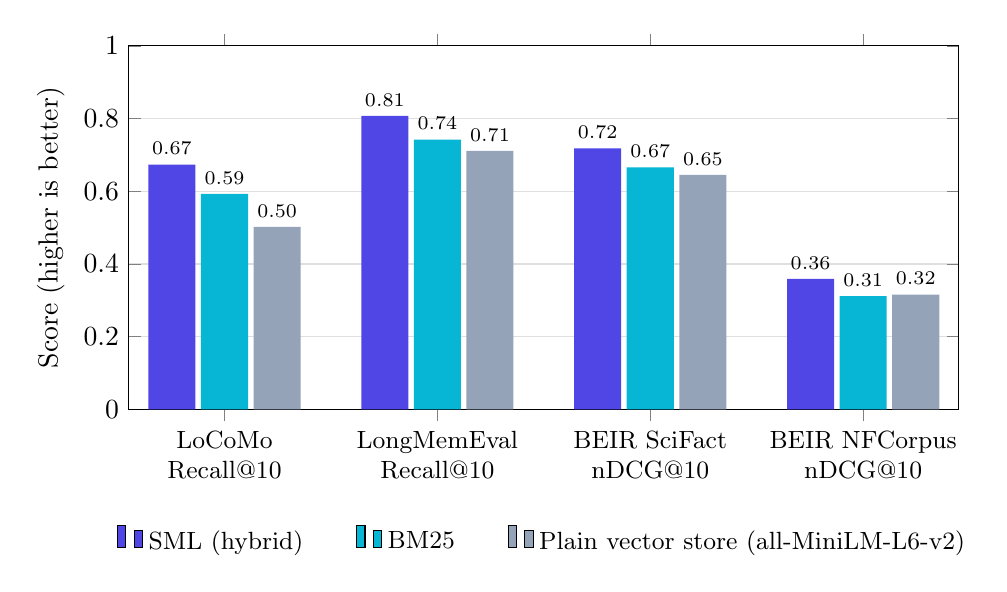
\begin{tikzpicture}
\begin{axis}[
  ybar, bar width=17pt, width=\textwidth, height=6.2cm,
  ymin=0, ymax=1.0, ylabel={Score (higher is better)},
  symbolic x coords={LoCoMo,LongMemEval,SciFact,NFCorpus}, xtick=data,
  xticklabels={{LoCoMo\\Recall@10},{LongMemEval\\Recall@10},{BEIR SciFact\\nDCG@10},{BEIR NFCorpus\\nDCG@10}},
  xticklabel style={align=center, font=\small}, enlarge x limits=0.15,
  ymajorgrids=true, grid style={gray!25},
  nodes near coords={\pgfmathprintnumber[fixed zerofill,precision=2]{\pgfplotspointmeta}},
  every node near coord/.append style={font=\scriptsize},
  legend style={at={(0.5,-0.3)}, anchor=north, legend columns=-1, draw=none, font=\small, /tikz/every even column/.append style={column sep=0.6cm}},
  legend cell align=left,
]
\addplot[fill=smlindigo, draw=none] coordinates {(LoCoMo,0.673) (LongMemEval,0.807) (SciFact,0.718) (NFCorpus,0.359)};
\addplot[fill=smlcyan, draw=none] coordinates {(LoCoMo,0.593) (LongMemEval,0.742) (SciFact,0.666) (NFCorpus,0.312)};
\addplot[fill=smlslate, draw=none] coordinates {(LoCoMo,0.502) (LongMemEval,0.711) (SciFact,0.645) (NFCorpus,0.316)};
\legend{\sys{} (hybrid), BM25, Plain vector store (all-MiniLM-L6-v2)}
\end{axis}
\end{tikzpicture}
\caption{Headline metric of each public benchmark, measured through \sys{}'s API, and two baselines on identical data.}
\label{fig:overview}
\end{figure}

Authorisation is only worth having if retrieval stays good. We ran three public benchmarks end to end through the API
(Figure~\ref{fig:overview}; full tables in the appendix).

\paragraph{LoCoMo}~\cite{maharana2024locomo} has very long multi-session conversations with annotated evidence turns; it
is the benchmark on which Mem0, Zep, LangMem and A-Mem report. Over the 1{,}535 answerable questions of the 10 released
conversations, \sys{}'s hybrid search reaches Recall@10 0.673, within 0.01 of the DRAGON retriever~\cite{lin2023dragon}
reported by the benchmark authors at every depth (Figure~\ref{fig:locomo}), although DRAGON has about three times as many
parameters and was evaluated on the full 50-conversation set. Its margin over BM25 is largest on multi-hop and open-domain
questions (+0.21 Recall@10), which paraphrase their evidence.

\begin{figure}[htbp]
\centering
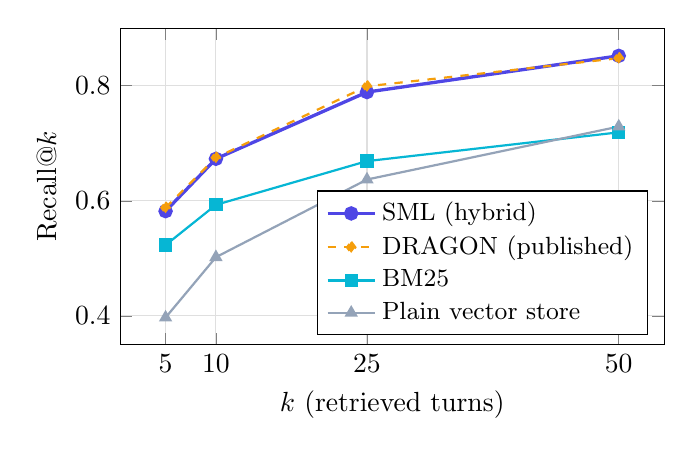
\begin{tikzpicture}
\begin{axis}[
  width=0.7\textwidth, height=5.6cm,
  xlabel={$k$ (retrieved turns)}, ylabel={Recall@$k$},
  xtick={5,10,25,50}, ymin=0.35, ymax=0.9, grid=major, grid style={gray!25},
  legend pos=south east, legend style={font=\small}, legend cell align=left,
]
\addplot[smlindigo, very thick, mark=*] coordinates {(5,0.582) (10,0.673) (25,0.789) (50,0.852)};
\addplot[smlamber, thick, dashed, mark=diamond*] coordinates {(5,0.588) (10,0.675) (25,0.799) (50,0.848)};
\addplot[smlcyan, thick, mark=square*] coordinates {(5,0.523) (10,0.593) (25,0.669) (50,0.719)};
\addplot[smlslate, thick, mark=triangle*] coordinates {(5,0.397) (10,0.502) (25,0.637) (50,0.729)};
\legend{\sys{} (hybrid), DRAGON (published), BM25, Plain vector store}
\end{axis}
\end{tikzpicture}
\caption{LoCoMo Recall@$k$ through \sys{}'s permission-checked API.}
\label{fig:locomo}
\end{figure}

\paragraph{LongMemEval}~\cite{wu2025longmemeval} gives each question its own chat history of about 48 sessions. Following
the official protocol on LongMemEval$_S$ (419 questions, 102{,}229 stored user messages; Recall@$k$ requires \emph{all}
evidence messages in the top $k$), \sys{} reaches Recall@10 0.807 against 0.742 for BM25 and 0.711 for the plain vector
store, and places all evidence within the top 50 for 97.4\,\% of questions. BM25 is marginally ahead on temporal and
user-fact questions, which repeat exact names and dates---the price of \sys{}'s conservative, document-local keyword
component (Section~\ref{sec:discussion}).

\begin{sloppypar}
\paragraph{BEIR}~\cite{thakur2021beir} measures zero-shot document retrieval. \sys{} scores nDCG@10 0.718 on SciFact and
0.359 on NFCorpus---above BM25, ColBERT~\cite{khattab2020colbert}, a BM25 plus cross-encoder pipeline and Chroma's default
embedder, and within 0.016 and 0.024 of OpenAI's hosted \texttt{text-embedding-3-small}, Mem0's default embedder.
\end{sloppypar}

\paragraph{Other memory layers.} Mem0, Zep, LangMem and A-Mem report LoCoMo \emph{answer accuracy} judged by an LLM
(Table~\ref{tab:mem0}) with the hosted GPT-4o-mini over all questions; \sys{}'s answer accuracy (RQ6) was measured with a
local open model on a sample, so it is comparable with the configurations we ran, not with these numbers. On
LongMemEval$_S$ Zep reports 71.2\,\% answer accuracy with GPT-4o (60.2\,\% for GPT-4o reading the full
history)~\cite{rasmussen2025zep}. None of these evaluations reports access-control leakage or auditability.

\begin{table}[htbp]
\centering
\small
\caption{LoCoMo results of other memory layers as published in the Mem0 paper~\cite{chhikara2025mem0} (GPT-4o-mini as
answerer and judge, all questions), and \sys{} as measured. Published latencies include network access to hosted services.
$^{\ddagger}$Gemma~4 8B (local) as answerer and judge on @@QA:n@@ sampled questions (RQ6): comparable with the configurations
we ran, not with the rows above.}
\label{tab:mem0}
\begin{tabularx}{\textwidth}{@{}Y>{\centering\arraybackslash}p{2.6cm}>{\centering\arraybackslash}p{3.2cm}>{\centering\arraybackslash}p{1.9cm}>{\centering\arraybackslash}p{2.0cm}@{}}
\toprule
System & Answer accuracy (LLM judge) & Search p50 / p95 & Context tokens & Leakage tested \\
\midrule
Full context (no memory layer) & 72.9\,\% & -- & 26{,}031 & -- \\
Mem0 with graph memory & 68.4\,\% & 476 / 657 ms & 3{,}616 & no \\
Mem0 & 66.9\,\% & 148 / 200 ms & 1{,}764 & no \\
Zep & 66.0\,\% & 513 / 778 ms & 3{,}911 & no \\
LangMem & 58.1\,\% & 17{,}990 / 59{,}820 ms & 127 & no \\
A-Mem & 48.4\,\% & 668 / 1{,}485 ms & 2{,}520 & no \\
\midrule
\textbf{\sys{} (hybrid)} & @@QA:sml_hybrid:accuracy:pct@@$^{\ddagger}$ & \best{83 / 186 ms} & $\approx$441 & \best{yes, 0 / 140} \\
\bottomrule
\end{tabularx}
\end{table}

\subsection{RQ6: Does better retrieval yield more correct answers?}
\label{sec:rq6}

\paragraph{Protocol.} We follow the protocol of the Mem0 paper~\cite{chhikara2025mem0}: an LLM answers each LoCoMo question
from the memories a system retrieves, and an LLM judge labels the answer CORRECT or WRONG against the gold answer, with the
adversarial category excluded. We make one substitution: instead of the hosted GPT-4o-mini, an open model that runs on the
laptop, Gemma~4~\cite{gemma4card} (\texttt{gemma4:latest}: 8.0B parameters, 4-bit quantisation, served by Ollama at
temperature 0), acts as both answerer and judge, as one model does in the Mem0 protocol. The answerer receives the top-10
memories of a configuration, each with its date, and is asked for a short answer; the judge prompt, like Mem0's, accepts
different wording and date formats. Because CPU generation takes about 25\,s per answer, we drew a stratified random
sample of 200 of the @@QA:total@@ answerable questions (proportional to the four categories, fixed seed) in random order and
evaluated the first @@QA:n@@ of them---@@QA:sml_hybrid:catn:single-hop@@ single-hop, @@QA:sml_hybrid:catn:temporal@@
temporal, @@QA:sml_hybrid:catn:multi-hop@@ multi-hop and @@QA:sml_hybrid:catn:open-domain@@ open-domain; the remaining
questions were not run within the available compute time, and because the order was random the evaluated questions are
themselves a random sample. Every evaluated question is answered under four contexts---\sys{}'s hybrid search, BM25, the plain vector store, and no memory---so the
configurations are compared on identical questions with the exact McNemar test~\cite{mcnemar1947}; intervals are 95\,\%
Wilson intervals~\cite{wilson1927}.

\begin{table}[htbp]
\centering
\small
\caption{LoCoMo answer accuracy with an LLM judge (Gemma~4 8B as answerer and judge, @@QA:n@@ stratified questions, top-10
memories as context). \emph{Evidence retrieved}: accuracy on the questions for which at least one annotated evidence turn
was among the ten memories. McNemar tests are paired against \sys{}.}
\label{tab:qa}
\begin{tabularx}{\textwidth}{@{}Y>{\centering\arraybackslash}p{1.7cm}>{\centering\arraybackslash}p{2.6cm}>{\centering\arraybackslash}p{1.3cm}>{\centering\arraybackslash}p{2.2cm}>{\centering\arraybackslash}p{2.2cm}@{}}
\toprule
Context given to the answerer & Accuracy $J$ & 95\,\% CI & Tokens & $J$ when evidence retrieved & McNemar vs \sys{} \\
\midrule
\sys{} hybrid search & \best{@@QA:sml_hybrid:accuracy:pct@@} & @@QA:sml_hybrid:ci_lo:pct@@--@@QA:sml_hybrid:ci_hi:pct@@ & @@QA:sml_hybrid:tokens@@ & @@QA:sml_hybrid:ev_hit:pct@@ & -- \\
BM25 & @@QA:bm25:accuracy:pct@@ & @@QA:bm25:ci_lo:pct@@--@@QA:bm25:ci_hi:pct@@ & @@QA:bm25:tokens@@ & @@QA:bm25:ev_hit:pct@@ & @@QA:p:bm25@@ \\
Plain vector store & @@QA:dense:accuracy:pct@@ & @@QA:dense:ci_lo:pct@@--@@QA:dense:ci_hi:pct@@ & @@QA:dense:tokens@@ & @@QA:dense:ev_hit:pct@@ & @@QA:p:dense@@ \\
No memory & @@QA:none:accuracy:pct@@ & @@QA:none:ci_lo:pct@@--@@QA:none:ci_hi:pct@@ & 0 & -- & @@QA:p:none@@ \\
\bottomrule
\end{tabularx}
\end{table}

\paragraph{Findings.} Answers grounded in \sys{}'s memories were judged correct for @@QA:sml_hybrid:accuracy:pct@@ of
the questions, against @@QA:bm25:accuracy:pct@@ with BM25, @@QA:dense:accuracy:pct@@ with the plain vector store and
@@QA:none:accuracy:pct@@ without memory (Table~\ref{tab:qa}); without retrieved context the model declined or guessed wrongly
on every question, so all answer quality here comes from memory. \sys{} is significantly more accurate than the plain vector
store: @@QA:b:dense@@ questions were answered correctly only with \sys{}'s context and @@QA:c:dense@@ only with the vector
store's (@@QA:p:dense@@). Its lead over BM25 (@@QA:b:bm25@@ against @@QA:c:bm25@@ such questions) is not significant at this
sample size (@@QA:p:bm25@@). The ordering follows retrieval: whenever at least one evidence turn was among the ten memories,
the three retrievers led to almost the same accuracy (@@QA:sml_hybrid:ev_hit:pct@@, @@QA:bm25:ev_hit:pct@@ and
@@QA:dense:ev_hit:pct@@), and \sys{} put evidence into the context for @@QA:sml_hybrid:ev_share:pct@@ of the questions against
@@QA:bm25:ev_share:pct@@ for BM25 and @@QA:dense:ev_share:pct@@ for the vector store. The differences in answer accuracy therefore
come from what each retriever puts into the context, not from how the answerer uses it.

\paragraph{Is the judge reliable?} We audited @@QA:verify:n@@ randomly drawn judgments by hand, comparing each generated
answer with the gold answer under the judge's own rubric. The judge agreed with the audit on @@QA:verify:agreement:pct@@ of
them (Cohen's $\kappa = @@QA:verify:cohen_kappa@@$~\cite{cohen1960}); of the disagreements, @@QA:verify:judge_more_lenient@@
credited a related but different answer and @@QA:verify:judge_stricter@@ rejected an equivalent one. LLM judges are known to be
lenient~\cite{zheng2023judging}, so the absolute accuracies are probably a few points high; because the judge never sees which
context produced an answer, there is no reason for this bias to differ between contexts. The audit labels are released with
the results. Since answerer, judge and sample differ from the Mem0 paper's, these accuracies rank the four contexts against
each other; they are not comparable with the published GPT-4o-mini numbers in Table~\ref{tab:mem0}.

\subsection{RQ7: What does governed retrieval cost?}
\label{sec:rq7}

Median client-side search latency stayed between 83 and 109\,ms from 35 to 102{,}229 memories, with p95 below 210\,ms
(Appendix, Table~\ref{tab:latency}); server-side time---query embedding, filtered vector search, full-text query,
per-candidate re-check, ranking, access counters and the audit write---was 62\,ms at the median on LoCoMo. Filtering inside
the index did not measurably change vector-search latency (RQ1). Creating a memory with duplicate and contradiction detection took 189\,ms
at the median; bulk import without duplicate detection reached 14--23 memories per second on the laptop CPU, bounded by
embedding.

% ================================================================ 7 discussion
\section{Discussion}
\label{sec:discussion}

\paragraph{Lessons for memory and vector-database designers.} (i) \emph{Push the policy into the index.} Filtered
approximate search matched exact authorise-before-rank at no measurable cost (RQ1), whereas rank-then-filter leaks through
result counts and loses recall; over-fetching recovers recall in practice but only raises the number of similar hidden
memories an attacker needs. (ii) \emph{Keep scores document-local, or compute statistics per principal.} Hybrid engines
that compute BM25 over the shared index leak through scores even when every returned item is authorised (RQ2).
(iii) \emph{Re-check against the system of record.} Vector payloads are replicas; permissions change. (iv) \emph{Name your
declassification points} and audit them.

\paragraph{Limitations.} \sys{}'s keyword component rewards only memories containing every query term, which keeps it
document-local but conservative; a BM25-weighted lexical ranking with statistics restricted to the readable set, fused with
the dense ranking~\cite{cormack2009rrf}, should close the gap on name- and date-heavy questions. Answer accuracy was
measured with a local 8B model on @@QA:n@@ sampled questions rather than with GPT-4o-mini on all of them, so its absolute
level is not comparable with published J scores, and the full-context baseline (about 21{,}000 tokens per question) was
not run on the CPU. Published results of other systems were not reproduced and come from different hardware, hosted
services and, for DRAGON and Stella, larger data. The in-house corpus is small and author-written, which is why the public
benchmarks were added. Latencies come from one laptop with co-located services, and rate limiting was disabled on the
benchmark process only. RNI as defined ignores timing; approximate indexes can, in principle, reveal hidden structure
through recall differences, which we measured but did not bound. Finally, \sys{} does not consolidate or summarise memories
with an LLM; LongMemEval reports that LLM-extracted fact keys add about 0.09 Recall@10.

\paragraph{Broader impact.} Shared agent memory concentrates organisational knowledge. Need-to-know retrieval, audit
trails and human conflict review make that concentration governable; they do not prevent an authorised agent from
misusing what it may read, nor protect against poisoned knowledge written by an authorised principal~\cite{zou2025poisonedrag}.

% ================================================================ 8 related work
\section{Related Work}
\label{sec:related}

\paragraph{Memory for LLM agents.} Generative Agents~\cite{park2023generative} and MemGPT~\cite{packer2023memgpt}
established retrieval-based long-term memory for a single agent. Mem0~\cite{chhikara2025mem0}, Zep~\cite{rasmussen2025zep},
LangMem~\cite{langmem2025} and A-Mem~\cite{xu2025amem} build production memory layers around LLM-based extraction and
evaluate answer accuracy on LoCoMo~\cite{maharana2024locomo} and LongMemEval~\cite{wu2025longmemeval}. They scope memory by
user, agent or project; \sys{} targets organisation-wide sharing under per-memory need-to-know rules and evaluates leakage.
Multi-agent frameworks such as AutoGen~\cite{wu2023autogen}, MetaGPT~\cite{hong2024metagpt} and CAMEL~\cite{li2023camel}
share context within a run; \sys{} acts as a persistent, governed blackboard~\cite{wooldridge2009mas} across runs and teams
(Appendix, Table~\ref{tab:related}).

\begin{sloppypar}
\paragraph{Privacy and security of retrieval-augmented generation.} Retrieval databases leak through generated
text~\cite{zeng2024goodbad} and membership inference~\cite{anderson2025membership}, and can be poisoned to steer
answers~\cite{zou2025poisonedrag}. These works study a single-owner corpus exposed to users of one application; we study
multi-principal corpora in which the retrieval step itself must respect per-item permissions, and we formalise what that
step may reveal.
\end{sloppypar}

\paragraph{Secure search over shared indexes.} B{\"u}ttcher and Clarke showed that a system-wide full-text index with
post-processing leaks file contents to users who lack read permission, and proposed a security model in which statistics
are computed over what the user may see~\cite{buettcher2005security}. Our Propositions~\ref{prop:post} and \ref{prop:stats}
carry this line of work to dense and hybrid retrieval for agents and measure both channels. Non-interference~\cite{goguen1982noninterference}
and language-based information flow~\cite{sabelfeld2003language} provide the underlying notion.

\paragraph{Filtered vector search.} Filtered-DiskANN~\cite{gollapudi2023filtered} and ACORN~\cite{patel2024acorn} make
approximate nearest-neighbour search efficient under label or arbitrary predicates, and vector databases such as Qdrant
evaluate payload filters inside HNSW~\cite{malkov2020hnsw}. \sys{} uses such filtering as a security mechanism and shows that it
is both RNI-preserving in practice and nearly free.

\paragraph{Retrieval models and access control.} Dense retrievers~\cite{reimers2019sbert,karpukhin2020dpr,lin2023dragon},
embedding models~\cite{xiao2023cpack,wang2020minilm}, BM25~\cite{robertson2009bm25}, late interaction~\cite{khattab2020colbert},
retrieval-augmented generation~\cite{lewis2020rag} and the BEIR and MTEB benchmarks~\cite{thakur2021beir,muennighoff2023mteb}
underlie our retrieval and evaluation; RBAC~\cite{sandhu1996rbac} and ABAC~\cite{hu2014abac} underlie our policy model.

% ================================================================ 9 conclusion
\section{Conclusion}
\label{sec:conclusion}

A shared memory is only as trustworthy as its most permissive retrieval path. We defined retrieval non-interference,
showed that the familiar rank-then-filter design and index-wide lexical statistics both violate it, and built \sys{},
a collective memory for multi-team agents in which authorisation happens before ranking, scores are document-local,
every result is re-checked, and knowledge is versioned, reviewed and audited. Controlled experiments confirmed each
proposition; end to end, no adversarial attempt leaked, sharing turned unanswerable cross-team questions into answered ones,
retrieval matched the benchmark authors' own retriever with a small local model, and answers written from \sys{}'s memories
were judged correct for @@QA:sml_hybrid:accuracy:pct@@ of sampled questions---significantly more often than with a plain vector
store (@@QA:dense:accuracy:pct@@) and ahead of BM25 (@@QA:bm25:accuracy:pct@@). Need-to-know and good recall are not in
tension: placed correctly, authorisation costs nothing.

\paragraph{Artifact.} The system, the benchmark harnesses (in-house, LoCoMo, LongMemEval, BEIR, and the placement
experiments) and all raw results are part of the project repository.

% ================================================================ references
\bibliographystyle{unsrtnat}
\bibliography{references}

% ================================================================ appendix
\clearpage
\appendix
\section{Additional Tables}

\begin{table}[htbp]
\centering
\small
\caption{Memory visibility levels.}
\label{tab:visibility}
\begin{tabular}{@{}ll@{}}
\toprule
Visibility & Readable by (besides the creator and administrators) \\
\midrule
\texttt{private} & nobody else; private memories cannot be shared \\
\texttt{team} & members of the owning team, plus explicit team or agent grants \\
\texttt{selected\_teams} & the owning team plus the explicitly allowed teams \\
\texttt{selected\_agents} & only the explicitly allowed agents \\
\texttt{organization} & every authenticated principal \\
\bottomrule
\end{tabular}
\end{table}

\begin{table}[htbp]
\centering
\small
\caption{Capabilities of related approaches ($\checkmark$ supported, $\sim$ partial / session-scoped / via extensions,
-- not addressed), assessed from the designs described in the cited papers and documentation.}
\label{tab:related}
\begin{tabularx}{\textwidth}{@{}>{\raggedright\arraybackslash}p{4.3cm}*{6}{>{\centering\arraybackslash}X}@{}}
\toprule
Approach & Persistent memory & Cross-team sharing & Semantic retrieval & Per-memory access control & Versions \& provenance & Security audit trail \\
\midrule
AutoGen, MetaGPT, CAMEL & $\sim$ & $\sim$ & $\sim$ & -- & -- & -- \\
Generative Agents, MemGPT & $\checkmark$ & -- & $\checkmark$ & -- & -- & -- \\
RAG over a vector store & $\checkmark$ & $\sim$ & $\checkmark$ & $\sim$ & -- & -- \\
Mem0 & $\checkmark$ & $\sim$ & $\checkmark$ & $\sim$ & $\sim$ & -- \\
Zep & $\checkmark$ & $\sim$ & $\checkmark$ & -- & $\sim$ & -- \\
\midrule
\textbf{\sys{} (this work)} & $\checkmark$ & $\checkmark$ & $\checkmark$ & $\checkmark$ & $\checkmark$ & $\checkmark$ \\
\bottomrule
\end{tabularx}
\end{table}

\begin{table}[htbp]
\centering
\small
\caption{LoCoMo evidence retrieval through \sys{}'s API (1{,}535 questions). Bold: best measured value per column.}
\label{tab:locomo}
\begin{tabular}{@{}lccccccc@{}}
\toprule
Configuration & R@5 & R@10 & R@25 & R@50 & Hit@1 & MRR & nDCG@10 \\
\midrule
\sys{} hybrid & \best{0.582} & \best{0.673} & \best{0.789} & \best{0.852} & \best{0.392} & \best{0.511} & \best{0.523} \\
\sys{} dense only & 0.561 & 0.657 & 0.783 & 0.848 & 0.352 & 0.478 & 0.494 \\
\sys{} keyword only (all terms) & 0.119 & 0.121 & 0.122 & 0.123 & 0.118 & 0.126 & 0.118 \\
BM25 & 0.523 & 0.593 & 0.669 & 0.719 & 0.345 & 0.450 & 0.463 \\
Plain vector store & 0.397 & 0.502 & 0.637 & 0.729 & 0.212 & 0.326 & 0.344 \\
Recency (last $k$ turns) & 0.002 & 0.010 & 0.034 & 0.078 & 0.001 & 0.005 & 0.004 \\
\midrule
\textit{DRAGON (published, 50 conv.)} & \textit{0.588} & \textit{0.675} & \textit{0.799} & \textit{0.848} & -- & -- & -- \\
\bottomrule
\end{tabular}
\end{table}

\begin{table}[htbp]
\centering
\small
\caption{LoCoMo Recall@10 by question category (number of questions).}
\label{tab:locomocat}
\begin{tabular}{@{}lcccc@{}}
\toprule
Configuration & Single-hop (841) & Temporal (320) & Multi-hop (282) & Open-domain (92) \\
\midrule
\sys{} hybrid & \best{0.733} & \best{0.736} & \best{0.488} & \best{0.473} \\
\sys{} dense only & 0.711 & 0.720 & 0.485 & \best{0.473} \\
BM25 & 0.699 & 0.688 & 0.277 & 0.267 \\
Plain vector store & 0.570 & 0.562 & 0.309 & 0.266 \\
\bottomrule
\end{tabular}
\end{table}

\begin{table}[htbp]
\centering
\small
\caption{LongMemEval$_S$ retrieval (419 questions, official protocol). Stella~V5 1.5B~\cite{stella2024} was evaluated by the
LongMemEval authors on LongMemEval$_M$, whose haystack is about ten times larger; it is a reference point only.}
\label{tab:lme}
\begin{tabular}{@{}lcccccc@{}}
\toprule
 & \multicolumn{5}{c}{Message level} & Session level \\
\cmidrule(lr){2-6}\cmidrule(l){7-7}
Configuration & R@5 & NDCG@5 & R@10 & NDCG@10 & R@50 & R@10 \\
\midrule
\sys{} hybrid & \best{0.637} & 0.663 & \best{0.807} & \best{0.708} & \best{0.974} & 0.907 \\
\sys{} dense only & \best{0.637} & 0.656 & 0.802 & 0.700 & \best{0.974} & \best{0.909} \\
BM25 & 0.628 & \best{0.664} & 0.742 & 0.693 & 0.840 & 0.783 \\
Plain vector store & 0.511 & 0.570 & 0.711 & 0.623 & 0.936 & 0.840 \\
\midrule
\textit{Stella V5 1.5B on $M$ (published)} & \textit{0.582} & \textit{0.481} & \textit{0.692} & \textit{0.512} & -- & \textit{0.783} \\
\bottomrule
\end{tabular}
\end{table}

\begin{table}[htbp]
\centering
\small
\caption{LongMemEval$_S$ message-level Recall@10 by question type (number of questions).}
\label{tab:lmetype}
\begin{tabular}{@{}lcccccc@{}}
\toprule
Configuration & Multi-session & Temporal & Knowl.\ update & User facts & Preferences & Assistant \\
 & (121) & (127) & (72) & (64) & (30) & (5) \\
\midrule
\sys{} hybrid & \best{0.711} & 0.732 & \best{0.958} & 0.953 & \best{0.800} & \best{1.000} \\
\sys{} dense only & \best{0.711} & 0.724 & \best{0.958} & 0.938 & \best{0.800} & \best{1.000} \\
BM25 & 0.562 & \best{0.748} & 0.931 & \best{0.969} & 0.500 & 0.800 \\
Plain vector store & 0.545 & 0.614 & 0.903 & 0.953 & 0.767 & \best{1.000} \\
\bottomrule
\end{tabular}
\end{table}

\begin{table}[htbp]
\centering
\small
\caption{BEIR nDCG@10. Upper block measured through the \sys{} API; lower block published on the same test sets (BEIR
paper~\cite{thakur2021beir} and MTEB results~\cite{muennighoff2023mteb}).}
\label{tab:beir}
\begin{tabular}{@{}llcc@{}}
\toprule
Retriever & Source & SciFact & NFCorpus \\
\midrule
\sys{} hybrid (bge-small-en-v1.5, local) & measured & \best{0.718} & \best{0.359} \\
\sys{} dense only & measured & 0.717 & 0.342 \\
BM25 (this evaluation) & measured & 0.666 & 0.312 \\
Plain vector store, all-MiniLM-L6-v2 (this evaluation) & measured & 0.645 & 0.316 \\
\midrule
OpenAI text-embedding-3-small (Mem0's default embedder) & MTEB & 0.734 & 0.383 \\
OpenAI text-embedding-ada-002 & MTEB & 0.727 & 0.370 \\
bge-small-en-v1.5 & MTEB & 0.713 & 0.343 \\
BM25 + cross-encoder re-ranker & BEIR & 0.688 & 0.350 \\
ColBERT & BEIR & 0.671 & 0.305 \\
BM25 (Elasticsearch) & BEIR & 0.665 & 0.325 \\
all-MiniLM-L6-v2 (Chroma's default embedder) & MTEB & 0.645 & 0.316 \\
TAS-B & BEIR & 0.643 & 0.319 \\
ANCE & BEIR & 0.507 & 0.237 \\
DPR & BEIR & 0.318 & 0.189 \\
\bottomrule
\end{tabular}
\end{table}

\begin{table}[htbp]
\centering
\small
\caption{LoCoMo answer accuracy by question category (Gemma~4 8B answerer and judge; number of evaluated questions). The
open-domain column has very few questions and is shown for completeness only.}
\label{tab:qacat}
\begin{tabular}{@{}lcccc@{}}
\toprule
Context & Single-hop (@@QA:sml_hybrid:catn:single-hop@@) & Temporal (@@QA:sml_hybrid:catn:temporal@@) & Multi-hop (@@QA:sml_hybrid:catn:multi-hop@@) & Open-domain (@@QA:sml_hybrid:catn:open-domain@@) \\
\midrule
\sys{} hybrid search & @@QA:sml_hybrid:cat:single-hop:pct@@ & @@QA:sml_hybrid:cat:temporal:pct@@ & @@QA:sml_hybrid:cat:multi-hop:pct@@ & @@QA:sml_hybrid:cat:open-domain:pct@@ \\
BM25 & @@QA:bm25:cat:single-hop:pct@@ & @@QA:bm25:cat:temporal:pct@@ & @@QA:bm25:cat:multi-hop:pct@@ & @@QA:bm25:cat:open-domain:pct@@ \\
Plain vector store & @@QA:dense:cat:single-hop:pct@@ & @@QA:dense:cat:temporal:pct@@ & @@QA:dense:cat:multi-hop:pct@@ & @@QA:dense:cat:open-domain:pct@@ \\
No memory & @@QA:none:cat:single-hop:pct@@ & @@QA:none:cat:temporal:pct@@ & @@QA:none:cat:multi-hop:pct@@ & @@QA:none:cat:open-domain:pct@@ \\
\bottomrule
\end{tabular}
\end{table}

\begin{table}[htbp]
\centering
\small
\caption{Client-side search latency of \sys{}'s hybrid mode through the API (milliseconds).}
\label{tab:latency}
\begin{tabular}{@{}lrcc@{}}
\toprule
Workload & Memories in the collection & p50 & p95 \\
\midrule
In-house benchmark (top 5) & 35 & 103 & 208 \\
LoCoMo (top 50) & 5{,}882 & 83 & 186 \\
BEIR NFCorpus (top 50) & 3{,}633 & 90 & 180 \\
BEIR SciFact (top 50, long abstracts) & 5{,}183 & 109 & 197 \\
LongMemEval$_S$ (top 50) & 102{,}229 & 84 & 189 \\
\bottomrule
\end{tabular}
\end{table}

\end{document}
